% -*- coding: utf-8 -*-
% !TEX program = xelatex
\documentclass{jnuthesis}
\usepackage{amsmath}
\usepackage{algorithmic}
\usepackage{array}
\usepackage{fixltx2e}
\usepackage{stfloats}
\usepackage{url}
\usepackage{multicol}
\usepackage{graphicx}
\usepackage{ctex}
\usepackage{subfigure}
\usepackage{float}
\usepackage{indentfirst}
\usepackage{booktabs}
\usepackage{lscape}
\usepackage{caption}
\usepackage{subfigure}
\usepackage{titlesec}\titleclass{\chapter}{straight}
\titleformat{\chapter}[hang]  {\huge\bfseries}{\arabic{chapter}}{1em}{}

\usepackage{listings}
\usepackage{xcolor} 


\definecolor{mygreen}{rgb}{0,0.6,0}
\definecolor{mygray}{rgb}{0.5,0.5,0.5}
\definecolor{mymauve}{rgb}{0.58,0,0.82}
\lstset{ %
	backgroundcolor=\color{white},   % choose the background color
	basicstyle=\footnotesize\ttfamily,        % size of fonts used for the code
	columns=fullflexible,
	breaklines=true,                 % automatic line breaking only at whitespace
	captionpos=b,                    % sets the caption-position to bottom
	tabsize=4,
	commentstyle=\color{mygreen},    % comment style
	escapeinside={\%*}{*)},          % if you want to add LaTeX within your code
	keywordstyle=\color{blue},       % keyword style
	stringstyle=\color{mymauve}\ttfamily,     % string literal style
	frame=shadowbox,
	rulesepcolor=\color{red!20!green!20!blue!20},
	% identifierstyle=\color{red},
	numbers=left, 
	numberstyle=\tiny,
	% escapeinside=' ',
	xleftmargin=2em,
	xrightmargin=2em, 
	aboveskip=1em
}

\begin{document}

\renewcommand{\title}{A thesis class for Jinan University} % 英文标题
\renewcommand{\biaoti}{基于GRU的股市预测}  % 中文标题
\renewcommand{\xueyuan}{国际能源学院}
\renewcommand{\zhuanye}{电气工程及其自动化}
\renewcommand{\xingming}{余思贤、周允康}
\renewcommand{\xuehao}{2018054439}
\renewcommand{\daoshi}{庄师强}
\renewcommand{\zuzhang}{苏日清}
\renewcommand{\zuyuanone}{余思贤}
\renewcommand{\zuyuantwo}{梁宗威}
\renewcommand{\zuyuanthree}{谭铭濠}
\renewcommand{\zuyuanxhone}{2018054439}
\renewcommand{\zuyuanxhtwo}{2018054439}
\renewcommand{\zuyuanxhthree}{2018054439}
\renewcommand{\zuzhangxh}{2018054439}

\titlepage





\chapter{课程设计的任务与要求}
\section{课程设计的任务}

\begin{enumerate}
	\item 熟悉MATLAB中深度学习工具箱的使用方法,喂入数据的方法,配置训练的方法,保存模型的方法和调用模型的方法;
	\item 能画出学习模型的基本框架,理解其基本原理;
	\item 基于GRU对中国石化的开盘股价进行预测。
\end{enumerate}




\section{课程设计的要求}
\begin{enumerate}
	\item 学会MATLAB软件的安装;
	\item 熟练掌握MATLAB的使用,掌握深度学习工具箱的使用;
	\item 能使用深度学习工具箱根据需求搭建神经网络,喂入数据,训练,得出模型并能调用;
	\item 通过调参使得模型能更好的贴合实际,打到更好的效果。
\end{enumerate}

\chapter{研究基础}
\section{序列数据神经网络}

\subsection{RNN网络}
循环神经网络(Recurrent Neural Network,RNN)是一种用于处理序列数据的神经网络。相比一般的神经网络来说,他能够处理序列变化的数据。比如某个单词的意思会因为上文提到的内容不同而有不同的含义,RNN就能够很好地解决这类问题。

一般来说,普通RNN网络形式如下:
\begin{align}
	h^{\prime}=&\delta(w_h h+w_i x+b^{h})\\
	 y=&\delta( w_o h^{\prime}+b^{y})
\end{align}


其中$ h^{\prime} $为传入下一节点的参数,$ y $常使用对$ h^{\prime} $进行唯独映射,然后使用$ softmax $进行分类得到所需的参数。


\begin{figure}[H]
	\centering
	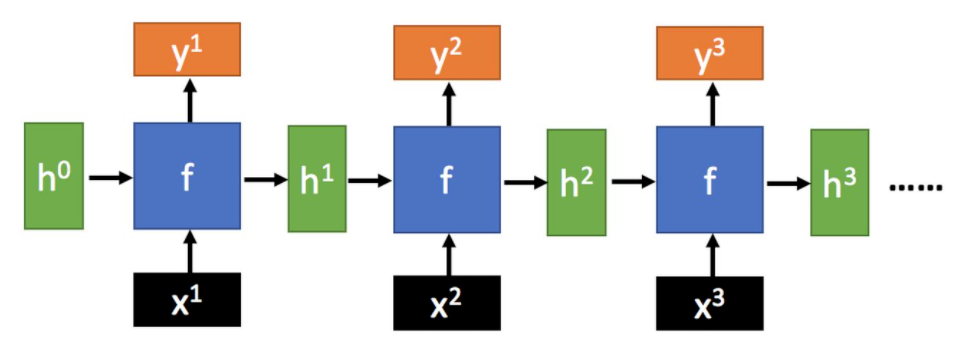
\includegraphics[width=\linewidth]{pic/screenshot001}
	\caption{多级RNN网络构成}
	\label{fig:screenshot001}
\end{figure}

\subsection{LSTM结构}

长短期记忆(Long short-term memory, LSTM)是一种特殊的RNN,主要是为了解决长序列训练过程中的梯度消失和梯度爆炸问题。简单来说,就是相比普通的RNN,LSTM能够在更长的序列中有更好的表现。

\begin{figure}[H]
	\centering
	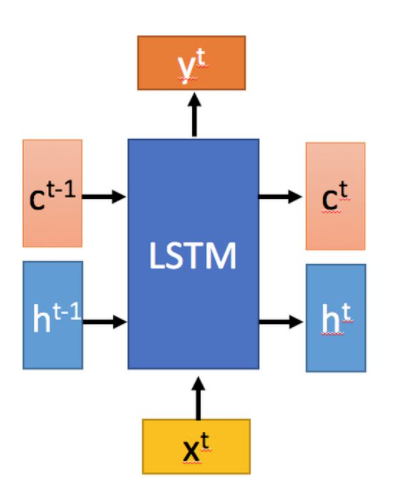
\includegraphics[width=0.3\linewidth]{pic/screenshot002}
	\caption{LTSM网络结构}
	\label{fig:screenshot002}
\end{figure}

LSTM网络的表达式如下:
\begin{align}
	 c^t=&z^f\odot c^{t-1}+z^{i}\odot z\\
	 h^{t}=&z^{o}\odot \tanh{c^{t}}\\
	 y^{t}=&\delta(W^{\prime}h^{t}+b^{y})
\end{align}

其中$ c^{t} $可以理解为长期记忆,主要是用来保存节点传递下来的数据的,每次传递会对某些维度进行“忘记”并且会加入当前节点所包含的内容;,$ h^{t} $则为短期记忆,仅保存了先前节点的信息。

\subsection{GRU网络}
GRU(Gate Recurrent Unit)是循环神经网络(Recurrent Neural Network, RNN)的一种。和LSTM(Long-Short Term Memory)一样,也是为了解决长期记忆和反向传播中的梯度等问题而提出来的。

GRU的输入输出结构与普通的RNN是一样的。
\begin{figure}[H]
	\centering
	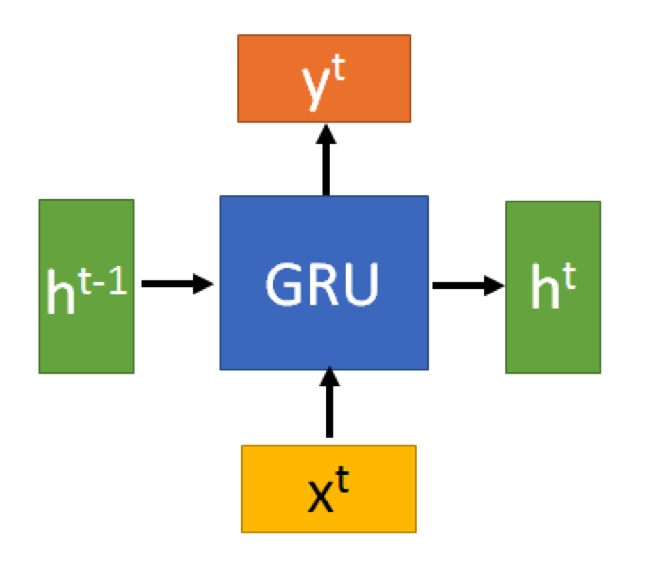
\includegraphics[width=0.3\linewidth]{pic/screenshot003}
	\caption{GRU的输入输出结构}
	\label{fig:screenshot003}
\end{figure}

其表达式为:
\begin{align}
	r^{t}=&\delta(x^{t}w^{xr}+h^{t-1}w^{hr}+b^{r})\\
	z^{t}=&\delta(x^{t}w^{xz}+h^{t-1}w^{hz}+b^{z})\\
	h^{\prime}=&\tanh{x^{t}w^{xr}+r^{t}\odot h^{t-1}w^{hh}+b^{h} }\\
	h^t=&(1-z)\odot h^{\prime}+z\odot h^{t-1}\\
	y^{t}=&\text{softmax}(h^{t}w^{hy}+b^{y})
\end{align}


GRU与LSTM相比,需要训练的参数较少,但也能达到与LSTM相近的效果。其训练的参数少,对硬件要求要求较低,因此本文采用GRU进行实现。
\section{训练数据的准备}
\subsection{数据采集}
这里使用Python爬取近16年中国石化(600028)的股市信息。

代码如下:

\begin{lstlisting} [language=Python]
import tushare as ts

df1 = ts.get_k_data('600028', ktype='D', start='2005-01-01', end='2021-10-16')

datapath1 = "./SH600028.csv"
df1.to_csv(datapath1)
\end{lstlisting}

得到了4032行数据,包括:时间、开盘价格、收市价、高位、低位、成交量以及股票代码。

\subsection{数据处理}

为使得模型更快收敛,并提高其准确性,对取得的数据进行归一化处理,公式如下:

\begin{equation}
x^*=\frac{X-X_{min}}{X_{max}-X_{min}}
\end{equation}


核心代码如下:
\begin{lstlisting} [language=Python]
from sklearn.preprocessing import MinMaxScaler

sc = MinMaxScaler(feature_range=(0, 1))  
training_set_scaled = sc.fit_transform(training_set)
test_set = sc.transform(test_set)
\end{lstlisting}

\subsection{数据标注}

为了实现股票预测,需要对训练用的数据进行标注。

GRU是根据过去预测未来,因此采用前两个月的数据进行对当日开盘价的预测。

取出后200日的数据作为测试数据,前3832日数据作为训练数据。

使用Python进行数据标注,并保存为txt文件,方便在MATLAB中进行读取调用。

标注核心代码如下:
\begin{lstlisting} [language=Python]
import pandas as pd

test_num=200
day=60

zhongshihua = pd.read_csv('./SH600028.csv')  
training_set = zhongshihua.iloc[0:len(zhongshihua) - test_num, 2:3].values
test_set = zhongshihua.iloc[len(zhongshihua) - test_num:, 2:3].values

for i in range(day, len(training_set_scaled)):  
	x_train.append(training_set_scaled[i - day:i, 0])
	y_train.append(training_set_scaled[i, 0])
\end{lstlisting}


\section{股市预测的Python实现}


先在Python中调用tensorflow框架进行本项目的实现,验证其可行性。

\begin{figure}[H]
	\centering
	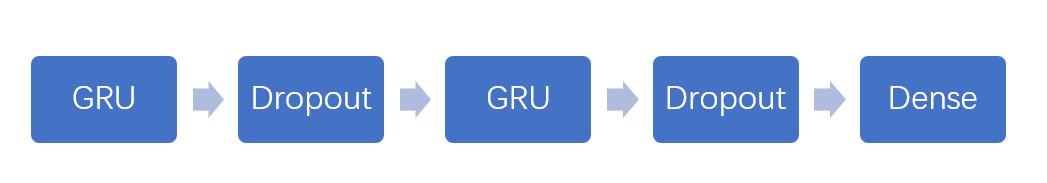
\includegraphics[width=1\linewidth]{pic/screenshot004}
	\caption{股市预测网络结构}
	\label{fig:screenshot004}
\end{figure}

核心代码如下(仅展示模型部分):
\begin{lstlisting} [language=Python]
import tensorflow as tf
from tensorflow.keras.layers import Dropout, Dense, GRU

model = tf.keras.Sequential([   
	GRU(512, return_sequences=True),
	Dropout(0.2),
	GRU(1024),
	Dropout(0.2),
	Dense(1)
	])
\end{lstlisting}


 第一层GRU:512个单元,每次返回$ h^t $参数;
 令其中20\%的单元休眠;
 第二层GRU:1024个单元,仅最后一次返回$ h^t $参数;
 令其中20\%的单元休眠;
 最后进行全链接输出。

在epochs=100,batch size=32的训练条件下,预测结果如图\ref{fig:screenshot005}:
\begin{figure}[H]
	\centering
	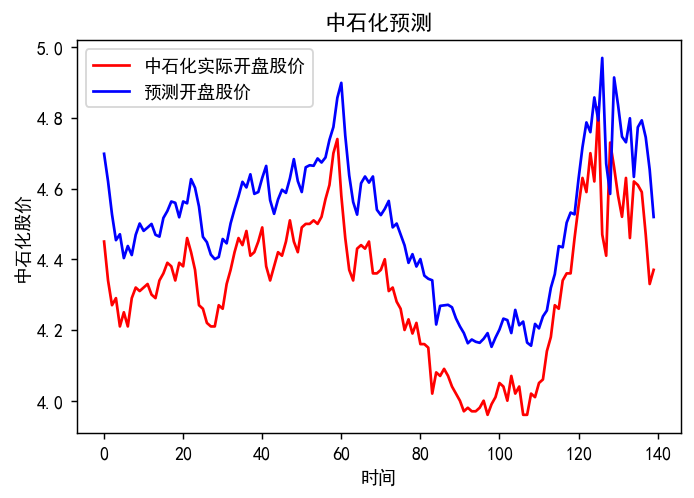
\includegraphics[width=0.7\linewidth]{pic/screenshot005}
	\caption{预测结果}
	\label{fig:screenshot005}
\end{figure}

可以看到:预测出的趋势与实际相比是较为准确的。

\chapter{股市预测的MATLAB实现}
\section{深度学习工具箱}

\textbf{这里你们来写,写完发字给我我打进来}
\section{在MATLAB中搭建GRU神经网络}

\textbf{搭一个图}

\section{喂入数据并训练}

\section{模型优化}


\subsection{效果评判}
后续测试模型中,我们采用茅台2005年1月1日到2021年3月20日的开盘股价作为训练集,为了节省时间,规定每一种模型均跑100Epoch。

我们使用如下指标进行模型效果评判:

\begin{enumerate}
	\item 计算茅台在2021年3月30日到2021年10月16日,共计200日的开盘股价预测数据,并与此200日的实际开盘股价计算确定系数。
	
	确定系数计算公式如下:
	\begin{equation}\label{r}
		r(X,Y)=\dfrac{\texttt{Cov}(X,Y)}{\sqrt{\texttt{Var}[X]\texttt{Var}[Y]}}
	\end{equation}
	式中,$ \texttt{Cov}(X,Y) $为X与Y的协方差,$ \texttt{Var}[X] $为X的方差,$ \texttt{Var}[Y] $为Y的方差。
	\item 计算模型计算速度,测试数据为:茅台在2021年3月30日到2021年10月16日的股价预测数据。计算速度测试中,时间计算单位为ms,一共跑100次,取平均值。
	\item 测试设备为联想拯救者R9000P(5800H+64G内存+RTX3070-8G)
	
	\item 综合评判公式:
	
	\textbf{先这么写着先,我并不确定这个可不可行}
	\begin{equation}\label{pingpan}
		s=\dfrac{r*10+T}{r*T}
	\end{equation}
\end{enumerate}

\subsection{优化方式}
\subsubsection{更改模型}
在3.3中,我们得到了粗略的结果,如图\ref{fig:screenshot005},其模型如图\ref{fig:screenshot004}。从结果中可以看出,虽然预测所得的结果趋势大致与实际情况近似,但其偏差还是较大。因此,在这一节中,我们更改了模型。其中更改的方向如下:

\begin{enumerate}
	\item 增减模型层数
	\item 调整 Dropout 单元的数量和 Dropout 的数值
	\item 调整 GRU 内神经元个数
	\item 在GRU中使用 sigmond 替换 tanh 
	\item 调整 beatch-size 都大小
\end{enumerate}

我们据此作出了10个新的模型,如表\ref{tab:my-table}所示。

% Please add the following required packages to your document preamble:
% \usepackage{graphicx}
\begin{table}[H]
	\caption{10种调参模型}
	\label{tab:my-table}
	\resizebox{\textwidth}{!}{%
		\begin{tabular}{lll}
			\hline
			序号 & \multicolumn{1}{c}{模型结构}                                             & 备注          \\ \hline
			1  & GRU(20)→Dropout(0.2)→GRU(20)→Dropout(0.2)→Dense                      &             \\
			2  & GRU(20)→Dropout(0.2)→GRU(20)→GRU(20)→Dropout(0.2)→Dense              &             \\
			3  & GRU(40)→Dropout(0.2)→GRU(80)→Dropout(0.2)→Dense                      &             \\
			4  & GRU(20)→Dropout(0.5)→GRU(20)→Dropout(0.5)→Dense                      &             \\
			5  & GRU(80)→Dropout(0.2)→GRU(160)→Dropout(0.2)→Dense                     &             \\
			6  & GRU(20)→GRU(20)→Dropout(0.2)→Dense                                   &             \\
			7  & GRU(20)→Dropout(0.2)→GRU(20)→Dropout(0.2)→Dense                      & 输出使用sigmoid \\
			8  & GRU(20)→Dropout(0.7)→GRU(20)→Dropout(0.7)→Dense                      &             \\
			9  & GRU(20)→Dropout(0.2)→GRU(20)→Dropout(0.2)→GRU(20)→Dropout(0.2)→Dense &             \\
			10 & GRU(20)→Dropout(0.2)→GRU(20)→GRU(20)→GRU(20)→Dropout(0.2)→Dense      &             \\ \hline
		\end{tabular}%
	}
\end{table}


下面进行模型效果评判,结果如下:

\begin{figure}[H]
	\centering
	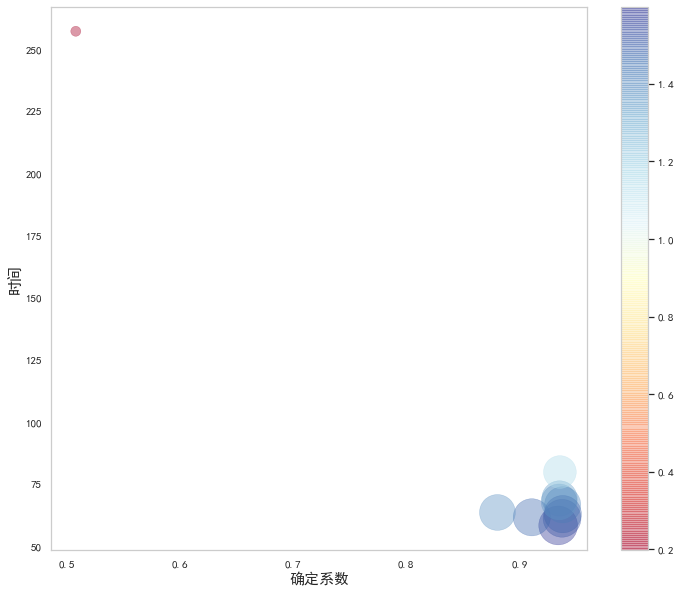
\includegraphics[width=0.5\linewidth,height=\textheight]{pic/screenshot014}
	\caption{}
	\label{fig:screenshot014}
\end{figure}




\subsubsection{每个GRU单元中偏置b初始化为1\cite{jozefowicz2015empirical}}

由上一小节,我们得出:模型???,即 xxxxx 的效果最好,因此此后都在此基础上修改。


\subsubsection{全链接层使用Highway Network代替\cite{srivastava2015highway}}




\subsubsection{调整batch size大小}

\section{结果}

\chapter{实验总结}


%\appendix
%\chapter*{结论}\addcontentsline{toc}{chapter}{\hspace{-1em}结论}
%
%
%
%
\chapter*{参考文献}\addcontentsline{toc}{chapter}{\hspace{-1em}参考文献}
\bibliographystyle{plain}
\bibliography{ref}



\end{document}
